% A separate graphics card against a shared memory pool.
% ---------------------------------------------------------------------------
% style.tex --- shared preamble for every figure in book/figures/tikz/
%
% One style for all figures: Latin Modern, thin black lines, a light grey
% fill, and one accent colour used only to mark what is untrusted or wrong.
% Build with scripts/build_figures.sh; see book/figures/README.md.
% ---------------------------------------------------------------------------
\documentclass[tikz,border=6pt]{standalone}
\usepackage[T1]{fontenc}
\usepackage{lmodern}
\usetikzlibrary{arrows.meta,positioning,shapes.geometric,calc,fit,backgrounds}

\hyphenpenalty=10000   % short lines in boxes: ragged, never hyphenated

\definecolor{lightgrey}{gray}{0.92}
\definecolor{accent}{HTML}{9B2D20}

\tikzset{
  every picture/.style={
    line width=0.6pt,
    font=\small,
    >={Stealth[length=5pt,width=4pt]},
    node distance=14pt and 24pt,
  },
  % shapes
  box/.style={draw, rectangle, inner xsep=8pt, inner ysep=5pt,
              minimum height=22pt, align=center},
  grey/.style={box, fill=lightgrey},
  rounded/.style={box, rounded corners=9pt},
  decision/.style={draw, diamond, aspect=2.4, inner sep=1.5pt, align=center},
  group/.style={draw, dashed, rounded corners=5pt, inner sep=7pt},
  % text
  tag/.style={font=\footnotesize, align=center, inner sep=2pt},
  note/.style={font=\footnotesize\itshape, align=center, inner sep=2pt},
  code/.style={font=\small\ttfamily},
  codetag/.style={font=\footnotesize\ttfamily, align=center, inner sep=2pt},
  title/.style={font=\small\scshape, align=center, inner sep=2pt},
  % lines
  arrow/.style={->},
  back/.style={->, dashed},
  thin/.style={line width=0.4pt, gray},
  % the one accent, for what is untrusted, wrong or missing
  bad/.style={accent},
  badbox/.style={box, draw=accent, text=accent},
}

\begin{document}
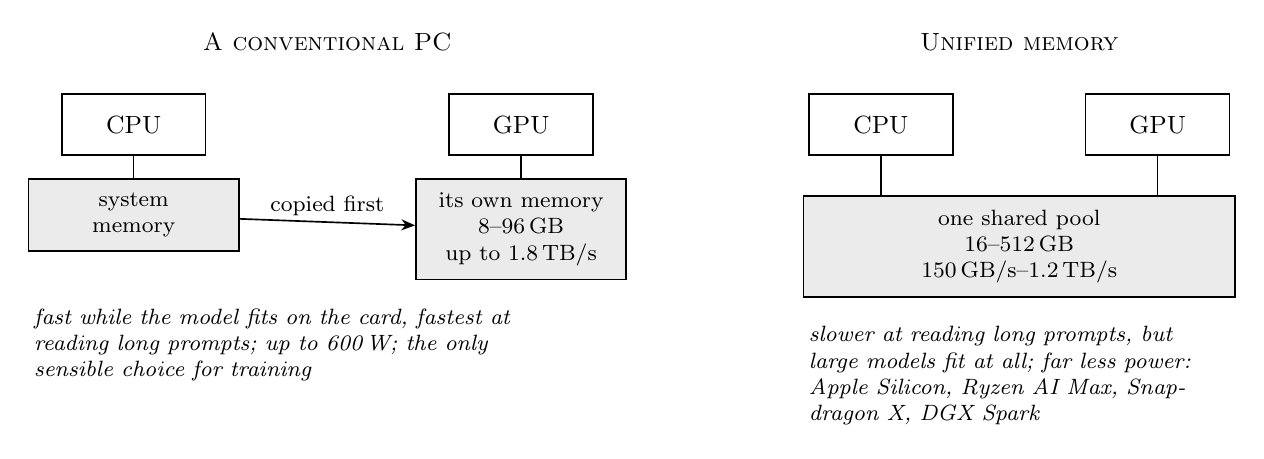
\begin{tikzpicture}[node distance=8pt and 20pt, chip/.style={box, minimum width=52pt}]
  % conventional
  \node[title] at (100pt,70pt) {A conventional PC};
  \node[chip] (cpu) at (30pt,40pt) {CPU};
  \node[grey, below=of cpu, text width=60pt, align=center, font=\footnotesize] (ram) {system\\memory};
  \node[chip] (gpu) at (170pt,40pt) {GPU};
  \node[grey, below=of gpu, text width=60pt, align=center, font=\footnotesize] (vram) {its own memory\\8--96\,GB\\up to 1.8\,TB/s};
  \draw (cpu) -- (ram); \draw (gpu) -- (vram);
  \draw[->] (ram) -- node[tag, above] {copied first} (vram);
  \node[note, anchor=north west, text width=176pt, align=left] at ([yshift=-8pt]ram.west |- vram.south)
    {fast while the model fits on the card, fastest at reading long prompts; up to 600\,W; the only sensible choice for training};
  % unified
  \node[title] at (350pt,70pt) {Unified memory};
  \node[chip] (cpu2) at (300pt,40pt) {CPU};
  \node[chip] (gpu2) at (400pt,40pt) {GPU};
  \node[grey, text width=140pt, align=center, font=\footnotesize] (pool) at (350pt,-4pt) {one shared pool\\16--512\,GB\\150\,GB/s--1.2\,TB/s};
  \draw (cpu2) -- (cpu2 |- pool.north); \draw (gpu2) -- (gpu2 |- pool.north);
  \node[note, below=8pt of pool.south west, anchor=north west, text width=140pt, align=left]
    {slower at reading long prompts, but large models fit at all; far less power: Apple Silicon, Ryzen AI Max, Snapdragon X, DGX Spark};
\end{tikzpicture}
\end{document}
